\documentclass[conference]{IEEEtran}
\usepackage{cite}
\usepackage{amsmath,amssymb,amsfonts}
\usepackage{algorithmic}
\usepackage{graphicx}
\usepackage{textcomp}
\usepackage{xcolor}
\usepackage{booktabs}
\def\BibTeX{{\rm B\kern-.05em{\sc i\kern-.025em b}\kern-.08em
    T\kern-.1667em\lower.7ex\hbox{E}\kern-.125emX}}

\begin{document}

\title{Design and Implementation of a Parallel Turbo Decoder for LTE in FPGA with Architectural Optimizations}

\author{\IEEEauthorblockN{Sai Vamshi}
\IEEEauthorblockA{\textit{EE-523 Digital VLSI Architecture Design} \\
\textit{Indian Institute of Technology (IIT) Mandi}\\
Mandi, India \\
}
}
\maketitle

\begin{abstract}
The increasing demand for high data rates in wireless communications, particularly in 3GPP-LTE Advanced systems, necessitates high-throughput baseband processing. The iterative nature of turbo decoding inherently poses a significant bottleneck to achieving peak system throughput. This paper details the hardware design and FPGA implementation of a parallel radix-4 Max-Log-MAP turbo decoder architecture. The proposed design reproduces a highly parallel M-BCJR architecture targeting the Zynq-7010 FPGA device, focusing on resolving architectural challenges such as memory contention, sliding window synchronization, and iterative latency. Through rigorous architectural mapping, including modulo-normalized Add-Compare-Select (ACS) units, contention-free interleaver addressing, and double-buffered internal memories, the decoder achieves significant throughput. Implementation results demonstrate mapping to the target FPGA at a 100 MHz clock constraint with timing closure. The design consumes approximately 79.5\% of the available LUTs and 56.6\% of BRAM resources on the Zynq-7010, establishing a robust baseline for further hardware optimization.
\end{abstract}

\begin{IEEEkeywords}
Turbo decoder, Max-Log-MAP, LTE, FPGA, Radix-4, M-BCJR
\end{IEEEkeywords}

\section{Introduction}
The 3rd Generation Partnership Project (3GPP) Long Term Evolution (LTE) standard employs turbo codes for forward error correction to achieve operation near the Shannon limit. While turbo codes offer exceptional error-correction performance, their iterative decoding algorithm involves severe data dependencies, presenting a primary bottleneck to achieving the high throughput required by modern wireless standards.

Traditional turbo decoding relies on the Bahl-Cocke-Jelinek-Raviv (BCJR) algorithm, which requires an entire frame to be received before decoding can commence. This introduces unacceptable latency and demands substantial memory for storing intermediate state metrics. To mitigate this, sliding-window techniques and parallel processing architectures have been introduced. However, scaling parallel decoders introduces significant challenges, primarily memory contention within the interleaver and the overhead of parallelization.

This paper presents the hardware reproduction and architectural evaluation of a parallel radix-4 turbo decoder architecture as described in contemporary literature~\cite{studer2011}, targeting an FPGA implementation. The key contributions of this work are as follows:
\begin{itemize}
    \item FPGA realization of a high-throughput parallel radix-4 M-BCJR turbo decoder.
    \item Architectural reproduction of critical functional units, avoiding multi-port BRAM conflicts through optimal folded memory mapping.
    \item Introduction of distinct algorithmic and architectural optimizations beyond reference literature for performance and routing enhancement.
    \item Comprehensive performance evaluation on a Xilinx Zynq-7010 FPGA, analyzing resource utilization, timing performance, algorithmic latency, and simulated BER parameters.
\end{itemize}

\section{Background}
\subsection{Turbo Decoding Principle}
An LTE turbo encoder consists of two parallel concatenated 8-state Recursive Systematic Convolutional (RSC) encoders, separated by a quadratic permutation polynomial (QPP) interleaver. The decoder structure mirrors this with two Soft-Input Soft-Output (SISO) decoders exchanging extrinsic information iteratively. The final bit decisions are made based on the intrinsic Log-Likelihood Ratios (LLRs) computed during the final iteration.

\subsection{Max-Log-MAP Algorithm}
The optimal Maximum A Posteriori (MAP) algorithm is hardware-prohibitive due to non-linear exponential operations. The Max-Log-MAP approximation algorithm substitutes the MAP computations with add-max operations in the log domain. The algorithm computes three primary metrics: forward state metrics ($\alpha$), backward state metrics ($\beta$), and branch metrics ($\gamma$).

\subsection{M-BCJR and Sliding Window}
To alleviate the memory requirements of storing $\alpha$ metrics for an entire block length (up to $K=6144$ bits in LTE), the sliding window (M-BCJR) approach is employed. The trellis is disjointed into smaller windows of length $M$. A dummy backward recursion is executed over subsequent windows to generate reliable initial $\beta$ values, eliminating the need for full-trellis metric storage.

\subsection{Parallel Decoding Strategy}
To achieve high throughput, the code block of length $K$ is uniformly divided into $N$ segments of length $S = K/N$. $N$ parallel SISO decoders operate concurrently on these segments. The QPP interleaver guarantees contention-free access, enabling parallel routing of extrinsic LLRs without memory collision.

\section{Proposed Architecture}

\subsection{Overall Architecture}
The global architecture consists of shared system memory, an interleaver/de-interleaver routing network, and $N$ parallel SISO decoder cores. The system instantiates parallel memories for systematic, parity, and extrinsic LLRs. To support the radix-4 throughput requirement of consuming two trellis steps per clock cycle, the global BRAMs are partitioned into even and odd arrays, effectively doubling the bandwidth. A global Finite State Machine (FSM) orchestrates the iterative decoding loop, executing 5.5 full iterations (11 half-iterations) per block. 

\begin{figure}[htbp]
\centerline{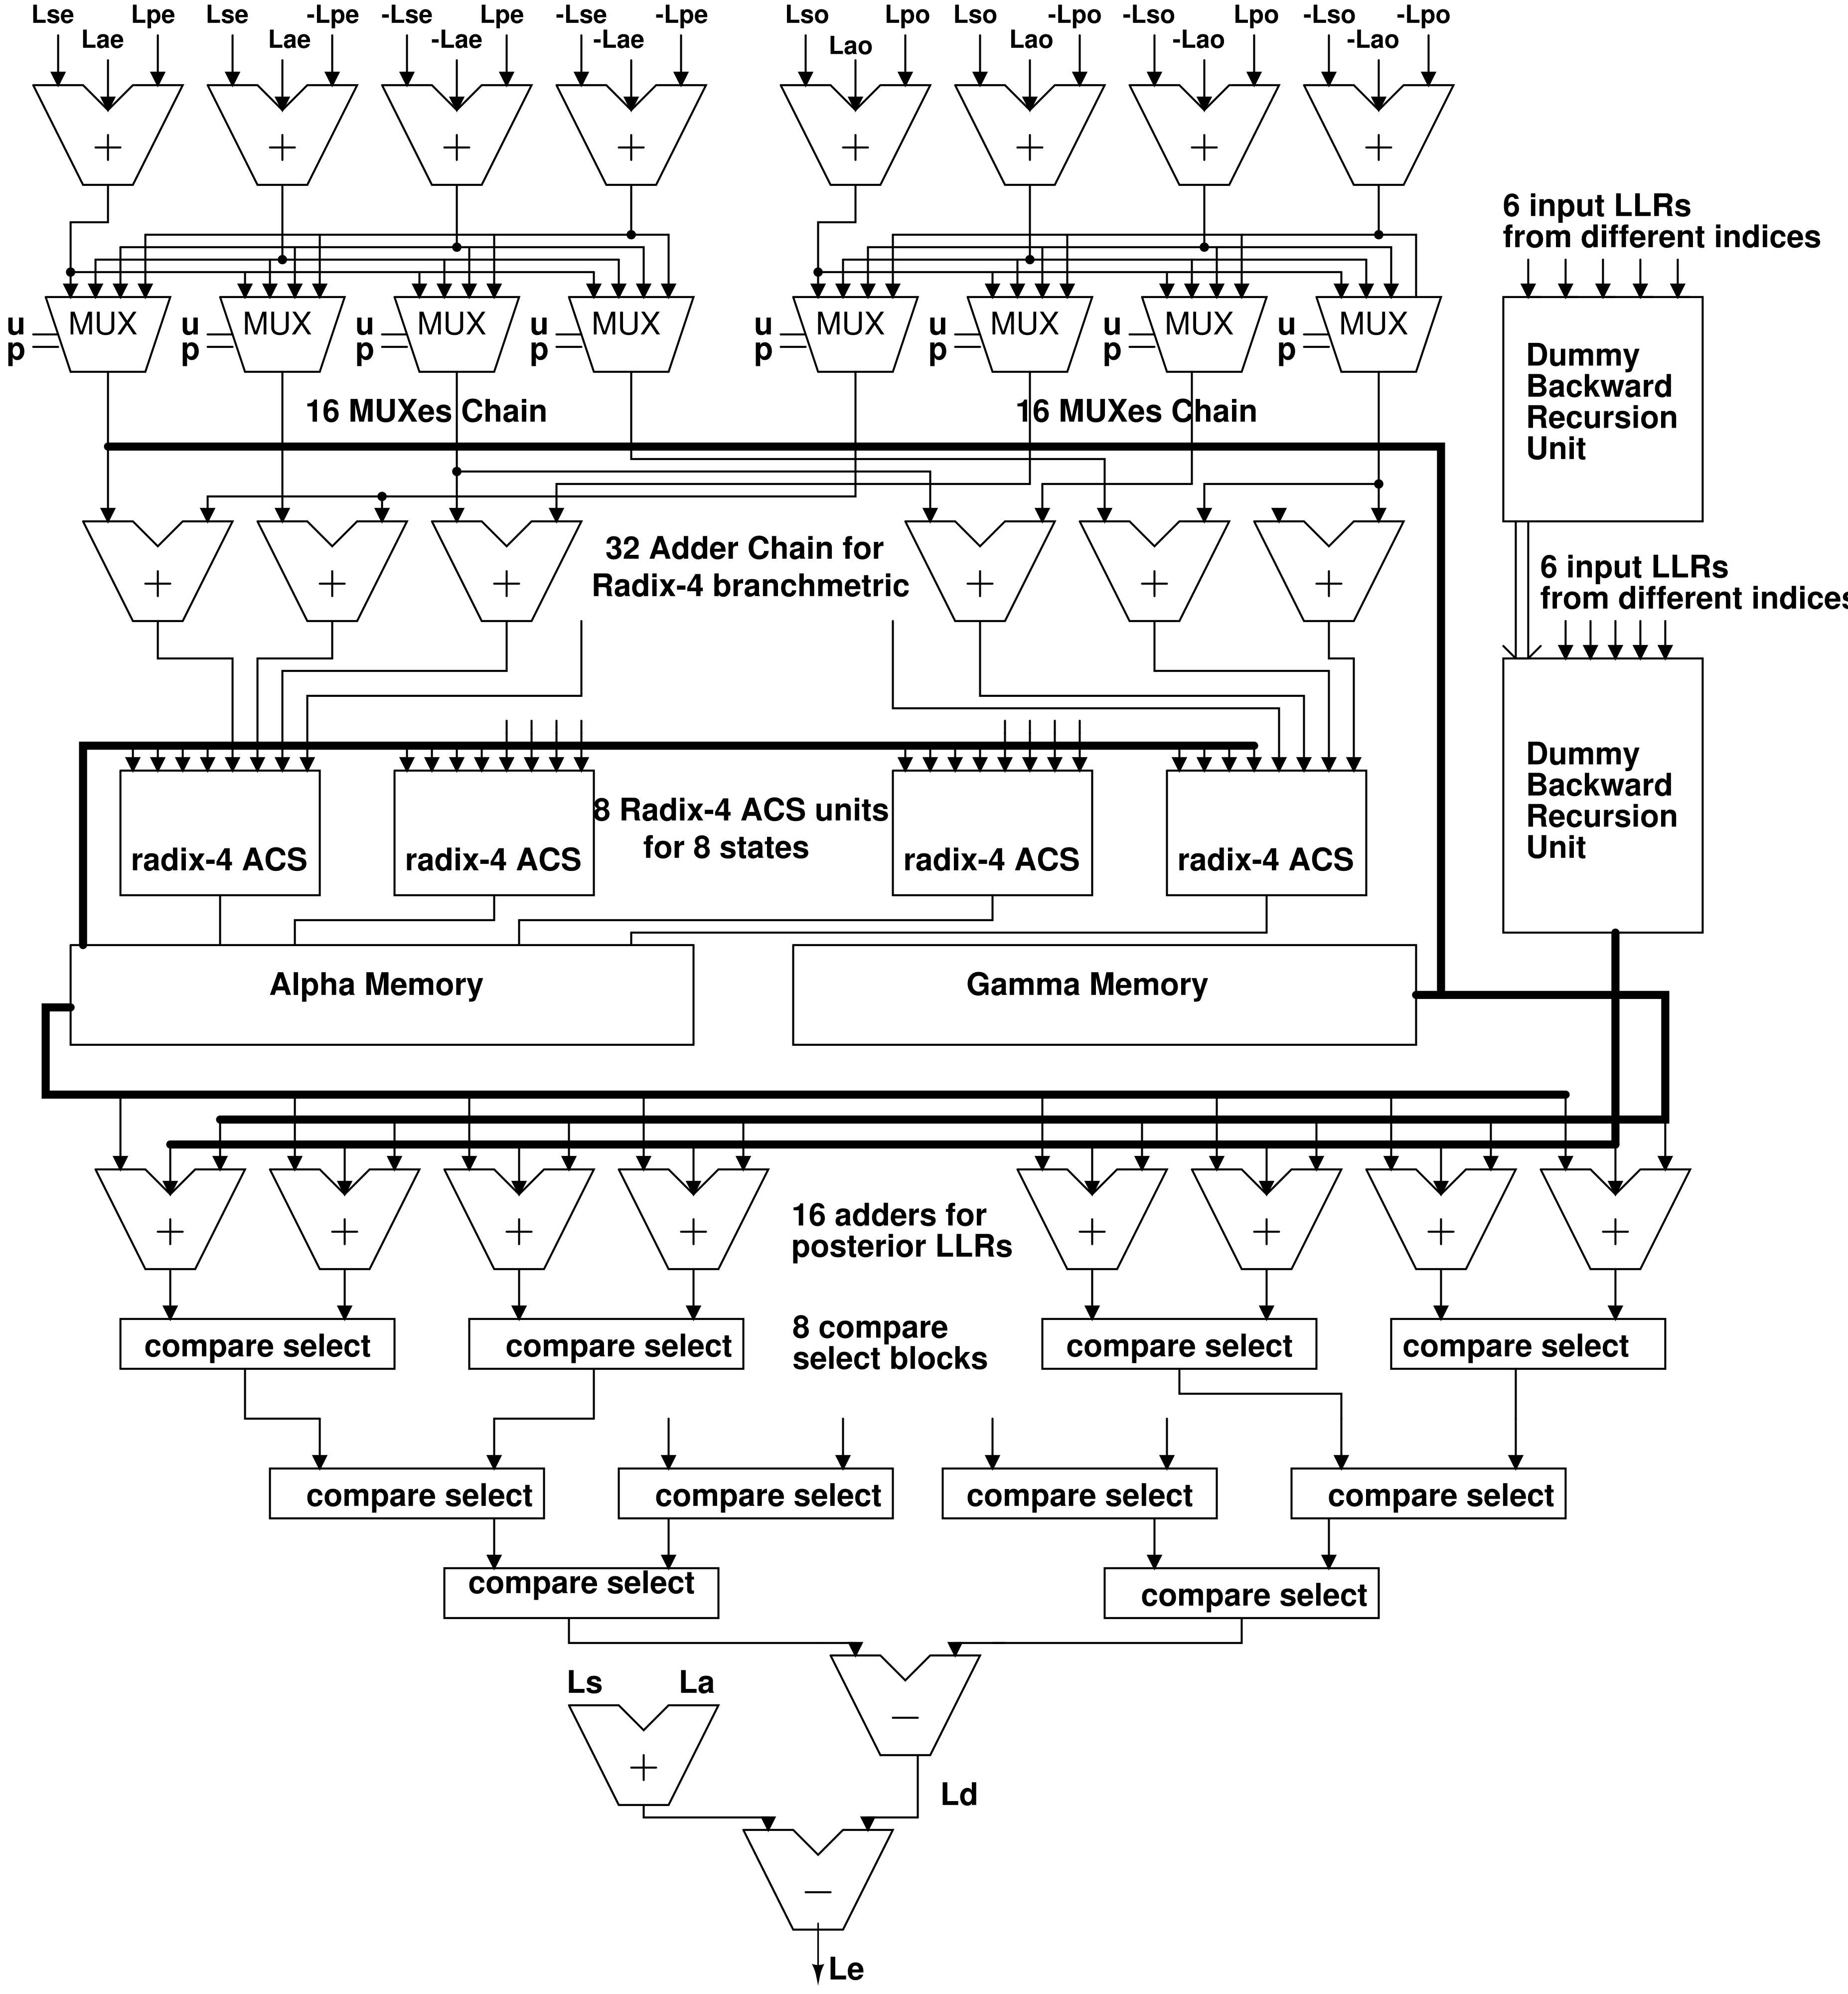
\includegraphics[width=\linewidth]{siso (1).png}}
\caption{Overall architecture of the parallel SISO M-BCJR core structure.}
\label{fig:bcjr_core}
\end{figure}

\subsection{SISO Decoder Design}
Each parallel SISO core implements a radix-4 Max-Log-MAP decoder processing 2 trellis steps per cycle. The core comprises three independent recursion pipelines operating concurrently:
\begin{enumerate}
    \item \textbf{Forward Recursion (FR):} Computes and stores forward state metrics ($\alpha$).
    \item \textbf{Backward Recursion (BR):} Navigates the trellis in reverse, utilizing stored branch metrics to compute trailing state metrics ($\beta$).
    \item \textbf{Dummy Backward Recursion (DBR):} Computes initialization metrics for the BR unit to seamlessly bridge adjacent sliding windows without performance degradation.
\end{enumerate}

The radix-4 Add-Compare-Select (ACS) unit is the arithmetic core. Instead of standard normalization which requires subtracting the minimum metric across all states, \textbf{modulo-normalization} is employed. By expanding the state metric precision to 10 bits and utilizing two's complement arithmetic, relative metric differences are correctly maintained under overflow conditions. Furthermore, the ACS logic natively flattens the evaluation by analyzing all six pairwise differences of the four candidate state metrics simultaneously. By examining the sign bits of these modulo-differences, the result vector directly indexes a 24-entry, 6-bit combinatorial Look-Up Table (LUT), resolving the 4-way classification cleanly without invoking cascaded binary tree comparators.

\begin{figure}[htbp]
\centerline{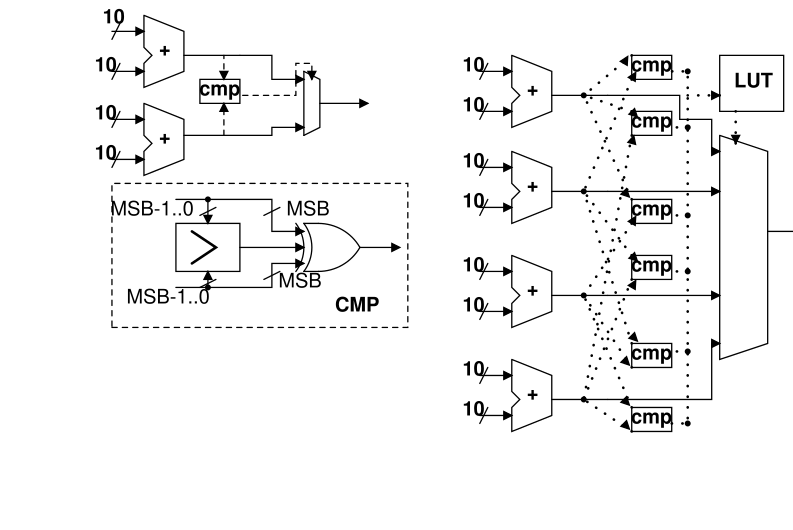
\includegraphics[width=\linewidth]{radix4.png}}
\caption{Radix-4 ACS computation structure with modulo comparator and LUT-based selection.}
\label{fig:radix_acs}
\end{figure}

\subsection{Memory Organization}
To sustain the concurrent operations of FR and BR within the sliding window datapath, the internal $\alpha$ and $\gamma$ memories are dual-buffered (ping-pong configuration). 
\begin{itemize}
    \item \textbf{$\alpha$-Memory:} Stores the 8 state metrics (10 bits each) outputted by the FR module.
    \item \textbf{$\gamma$-Memory:} Stores branch metrics arrayed as 32 metrics (7 bits each) derived by the radix-2 preprocessing block.
\end{itemize}
The FR array writes to Bank A while the BR array simultaneously reads from Bank B. The banks alternate at the window boundary. Distributed RAM (LUTRAM) is preferred over BRAM for these internal structures due to the small required depth ($M/2 = 15$ entries) and the necessity for simultaneous localized access.

\subsection{Interleaved Memory Hazard Management}
Operating parallel processing over shared extrinsic arrays necessarily exposes cyclic collision hazards across the read-fetch and interleaved write-back pipelines. The top-level finite control engine orchestrates a proactive 5-stage collision awareness protocol. An explicit stall-detection boundary continuously evaluates subsequent fetch targets against current dynamic permutations awaiting write-commit. Detected collisions temporarily arrest the central recursive arrays, invoking an isolated read reissue. This tightly couples extrinsic spatial coherence with just a 1-cycle penalty without inducing artificial trellis transitions or disrupting sliding window progression.

\subsection{Proposed Algorithmic and Architectural Optimizations}
To surpass the boundaries of standard reference designs and tailor the implementation tightly around the target Zynq-7010 fabric, several foundational optimizations were distinctly introduced beyond conventional literature baselines.

\begin{itemize}
    \item \textbf{Algorithmic Max-Log-MAP Upgrade via Correlation Factor:} Traditional Max-Log-MAP incurs a fundamental performance erosion due to the harsh max-approximation of logarithmic summations. To bridge this gap towards optimal MAP characteristics while preserving combinational simplicity, an algorithmic enhancement was integrated by appending an explicit mathematical correlation factor during branch metric and posterior LLR computations. Embedding this dynamic correlation logic fundamentally compensates for the structural biases encountered during decoding iterations, enhancing the trajectory natively within the state metric loops.
    
    \item \textbf{Parallelism Over Iterative Decomposition in Networking:} Standard concurrent implementations invoke massive $O(N \log^2 N)$ master-slave Batcher sorting networks to prevent interleaving memory multiplex collision at large $N$ blocks. By deliberately prioritizing raw parallelism and strictly anchoring $N=2$, the design dismisses dense iterative decompositions. Consequently, the conventionally exhaustive master-slave routing fabric natively collapses into a vastly simplified 2-element bipartite crossbar. This directly circumvents combinatorial routing hazards and frees crucial slice utilization properties.

\begin{figure}[htbp]
\centerline{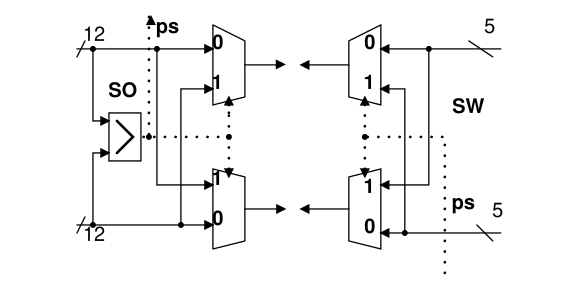
\includegraphics[width=\linewidth]{master_slave.png}}
\caption{Master-slave permutation network used for folded interleaved memory routing.}
\label{fig:master_slave}
\end{figure}

    \item \textbf{ROM/LUT QPP Interleaver Replacement:} Recursive algebraic processing of the comprehensive LTE interleaver polynomials poses severe combinational latencies when mapped strictly to structural DSP modules. The proposed architecture entirely substitutes recursive algorithmic configurations with direct chronological ROM/LUT look-up tables. By transferring the static polynomial properties of an explicit length constraint directly into fast distributed dual-port block RAM templates, identical concurrent cycle delivery is efficiently guaranteed decoupled from any arithmetic delay ceilings.
\end{itemize}

\section{Windowing Timing Waveforms}
At 100 MHz, one clock cycle is 10 ns. With radix-4 processing, each computation consumes two trellis bits; hence a window of $M=30$ contains 15 radix-4 steps.

\subsection{Single-Window Radix-4 Timing}
Fig.~\ref{fig:radix4_window_waveform} shows one complete window using \texttt{c0\_fr\_addr[11:0]}, \texttt{c0\_br\_addr[11:0]}, \texttt{c0\_dbr\_addr[11:0]}, and \texttt{c0\_llr\_req}. In steady state, FU computes $\alpha$ for $w_i$, BU computes $\beta$ for $w_{i-1}$, and DBU prepares $\beta$ for $w_{i+1}'$. The LLR request pulses once per radix-4 pair. Non-interleaved operation takes 5 cycles per pair, or 75 cycles per window. Interleaved operation adds one master-slave routing cycle, giving 6 cycles per pair, or 90 cycles per window; the QPP address and permutation rows show this routing overhead.

\begin{figure*}[!t]
\centerline{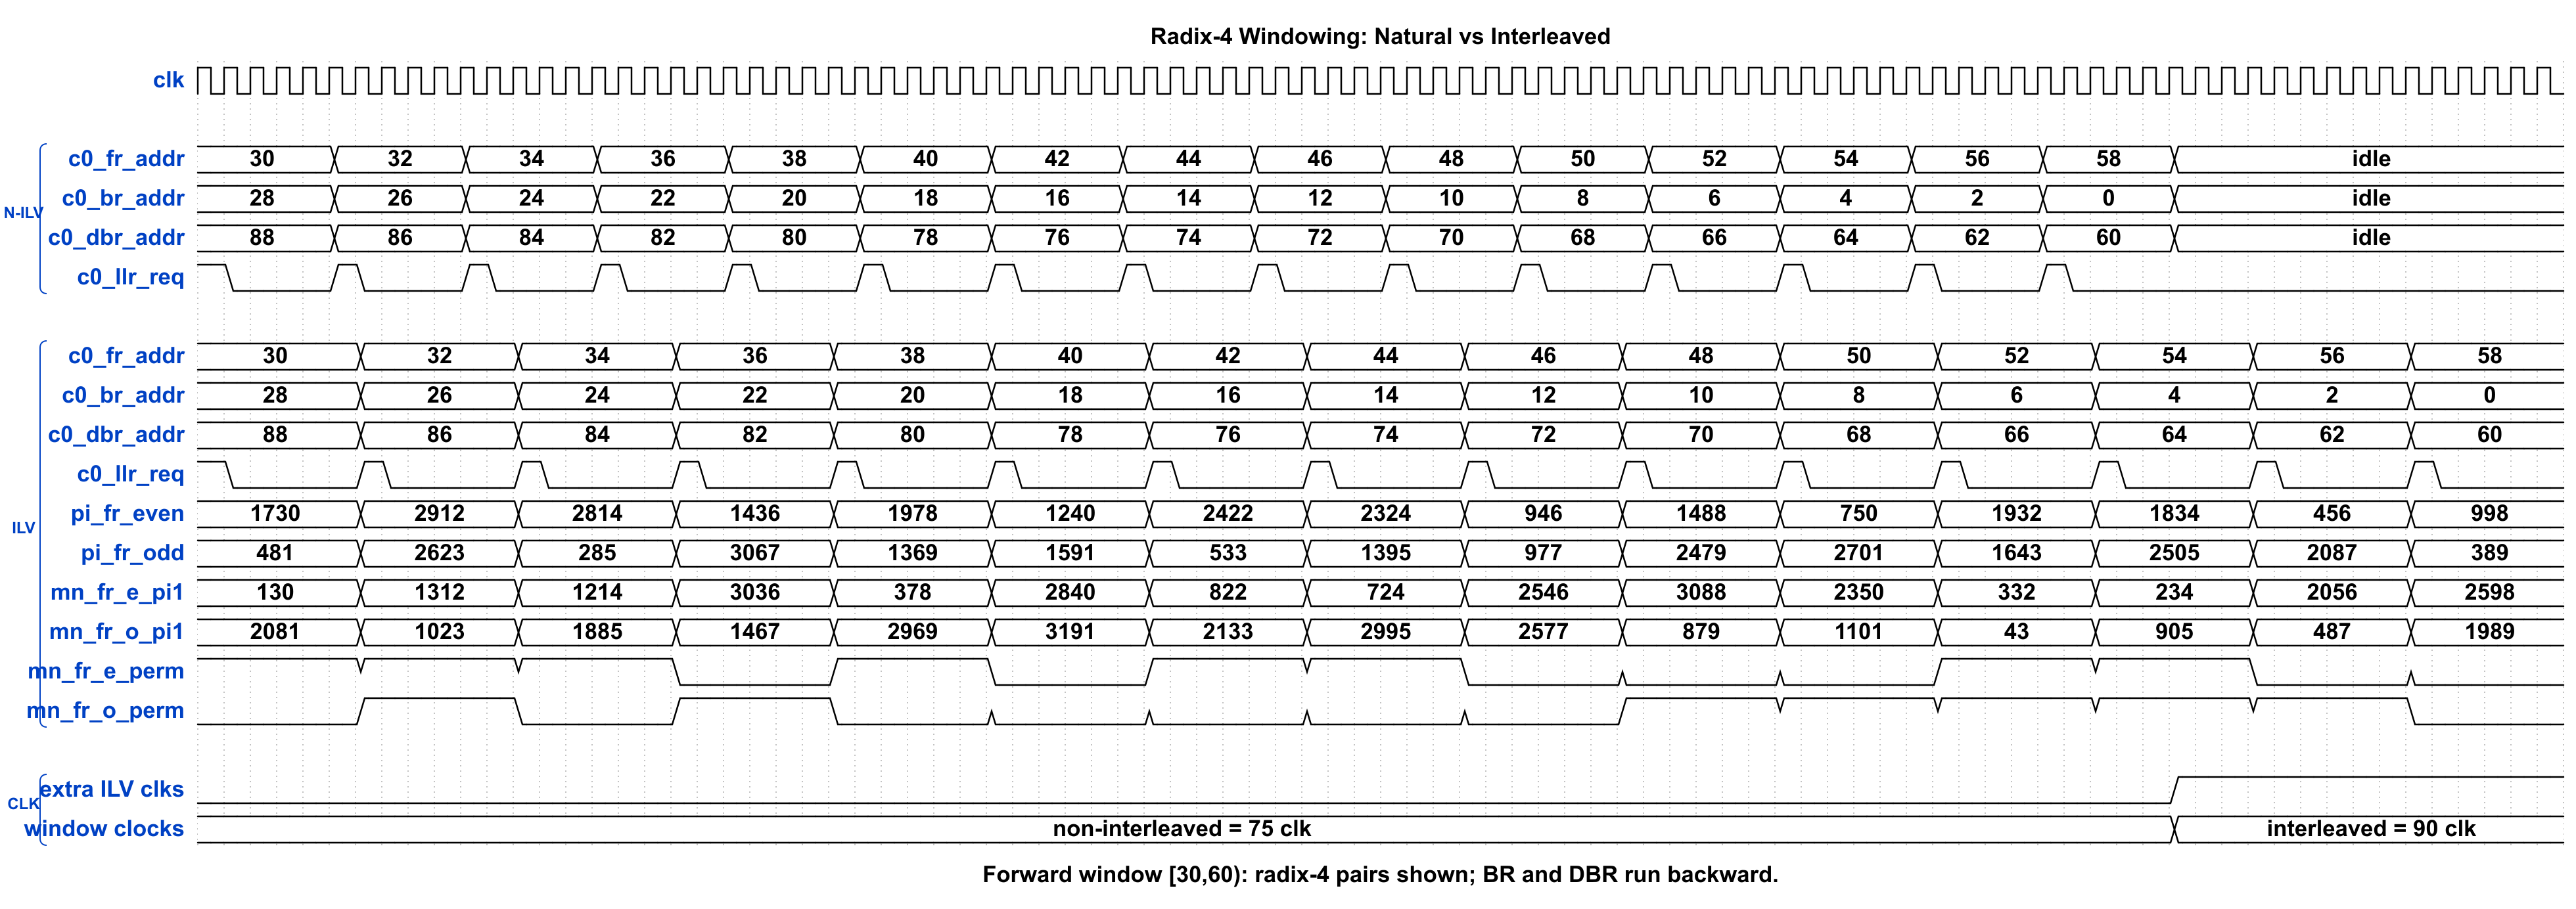
\includegraphics[width=\textwidth]{windowing_radix4_wavedrom.png}}
\caption{Single-window radix-4 timing comparing non-interleaved and interleaved operation.}
\label{fig:radix4_window_waveform}
\end{figure*}

\subsection{Two-SISO Boundary Window Flow}
Fig.~\ref{fig:siso_window_schedule_waveform} compresses the first, middle, and last slots for C0/SISO1 and C1/SISO2. Each block is one complete window slot. The steady-state rule is FU=$w_i$, BU=$w_{i-1}$, and DBU=$w_{i+1}'$. Only the boundary slots differ: C1/SISO2 begins with a dummy-forward warm-up, C0/SISO1 uses DBU $w_{54}'$ to reach the C1 boundary, and the final SISO segment ends with the terminal BU condition.

\begin{figure*}[!t]
\centerline{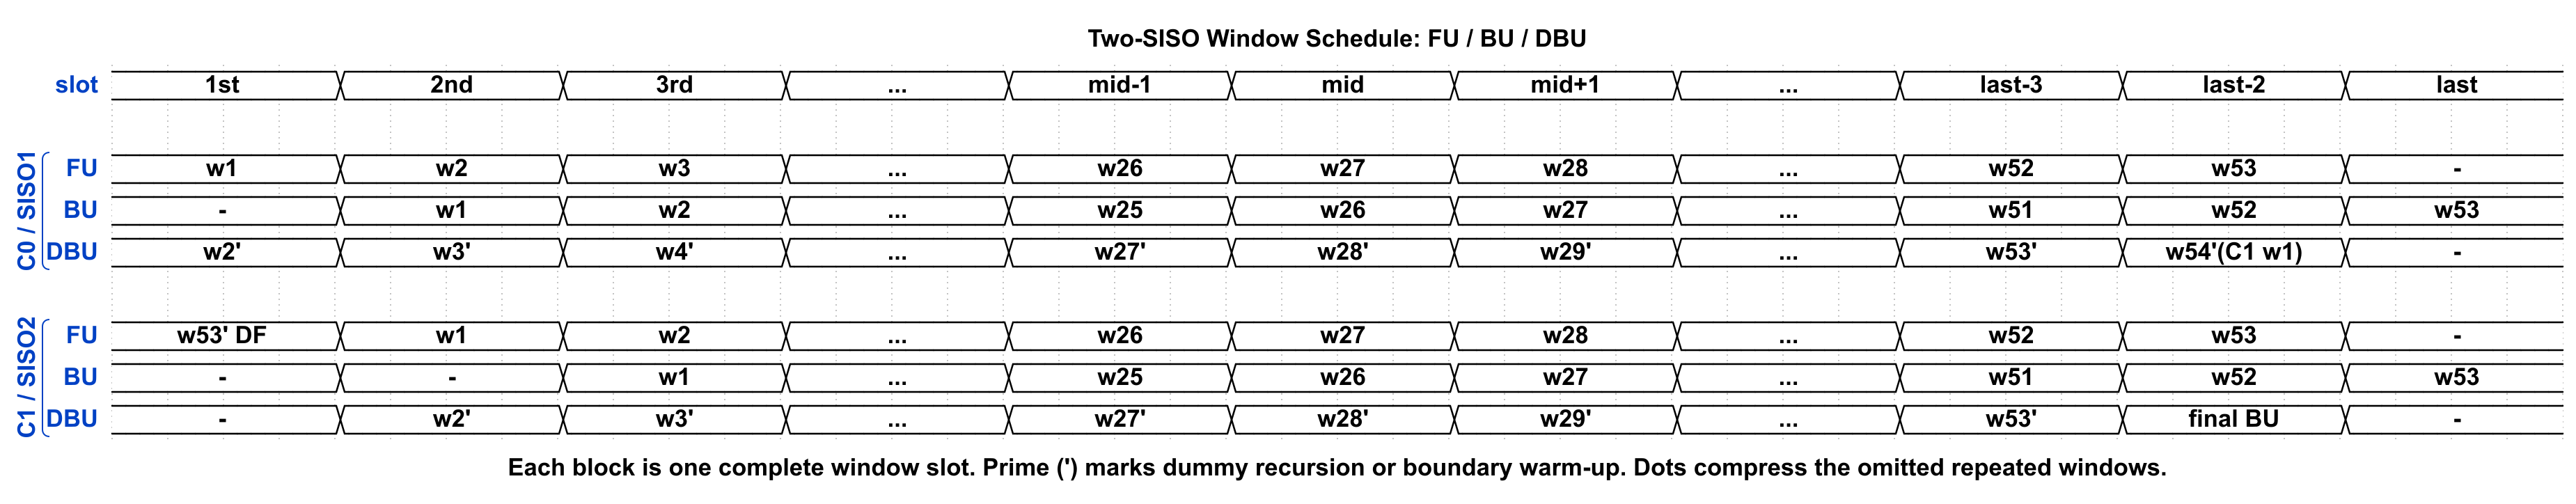
\includegraphics[width=\textwidth]{window_schedule_c0_c1_wavedrom.png}}
\caption{Two-SISO window schedule at the initial, steady-state, and final boundary slots.}
\label{fig:siso_window_schedule_waveform}
\end{figure*}

\section{FPGA Implementation}
The hardware description was captured using Verilog-2001 and mapped to the Xilinx Zynq-7010 (xc7z010clg400-1) target using the Vivado 2024.2 design suite. The RTL was structurally divided to allow hierarchical synthesis. Dedicated block RAM (BRAM36) cells were inferred for the global systematic, parity, and extrinsic buffering arrays. DSP elements were explicitly constrained to avoid unnecessary inference, preserving slices for the arithmetic logic dominant ACS blocks. Extensive timing constraints and pipelining directives were employed around the radix-4 LLR computation tree to satisfy setup violations typical in complex signed-magnitude max-trees. 

\section{Results and Verification}

\subsection{Resource Utilization}
The post-implementation resource utilization for the parallel radix-4 decoder ($N=2$, $K=3200$) targeted for the Zynq-7010 FPGA is summarized in Table~\ref{tab:utilization}.

\begin{table}[htbp]
\caption{Post-Implementation Resource Utilization (Zynq-7010)}
\begin{center}
\begin{tabular}{|c|c|c|c|}
\hline
\textbf{Resource} & \textbf{Utilized} & \textbf{Available} & \textbf{Utilization (\%)} \\
\hline
LUT & 13,999 & 17,600 & 79.54\% \\
\hline
LUTRAM & 384 & 6,000 & 6.40\% \\
\hline
FF & 2,179 & 35,200 & 6.19\% \\
\hline
BRAM & 34 & 60 & 56.67\% \\
\hline
DSP & 4 & 80 & 5.00\% \\
\hline
\end{tabular}
\label{tab:utilization}
\end{center}
\end{table}

The utilization metrics reflect the dense combinatorial nature of the parallel ACS architectures. The total LUT consumption approaches an 80\% ceiling, signifying the logic limits of the Zynq-7010 chassis for highly parallel baseband IP. Internal data buffering accounts for the minimal LUTRAM instantiation.

\subsection{Timing Performance}
The final post-route timing report meets all user-specified timing constraints at a 10 ns clock period. Debug-hub BSCAN/TCK paths were excluded from decoder-path interpretation because they belong to Vivado debug infrastructure. The filtered decoder timing is summarized in Table~\ref{tab:timing_summary}.

\begin{table}[htbp]
\caption{Filtered Timing Verification Summary}
\begin{center}
\scriptsize
\begin{tabular}{@{}p{0.43\linewidth}p{0.50\linewidth}@{}}
\toprule
\textbf{Metric} & \textbf{Value} \\
\midrule
Clock/status & 100 MHz, timing met \\
Setup & WNS/TNS = 0.230/0 ns; 0 failing endpoints \\
Hold & WHS/THS = 0.030/0 ns; 0 failing endpoints \\
Pulse width & WPWS/TPWS = 3.750/0 ns; 0 failing endpoints \\
Data paths & Setup: DBR ACS-to-ACS, 9.752 ns (3.761 logic + 5.991 route), 0.230 slack. Hold: LLR stage-to-stage, 0.417 ns (0.209 logic + 0.208 route), 0.030 slack. \\
Min hold path & Shortest hold data path is FR alpha-write to alpha memory: 0.209 ns (0.141 logic + 0.068 route), 0.049 ns slack. \\
I/O note & \texttt{btn[3:0]} and \texttt{led[3:0]} lack explicit I/O delays. \\
\bottomrule
\end{tabular}
\label{tab:timing_summary}
\end{center}
\end{table}

\subsection{Throughput}
For the current block length $K=3200$, the throughput is computed from the measured cycle count $C$ as
\begin{equation}
T_h = \frac{K \times F_{clk}}{C}
\end{equation}

At 100 MHz, the 11-iteration non-interleaved latency of 7175 cycles gives 44.60 Mbps. The interleaved latency of 8015 cycles gives 39.93 Mbps. Including input loading, eight load phases of 802 cycles add 6416 cycles, giving end-to-end throughputs of 23.55 Mbps and 22.17 Mbps for non-interleaved and interleaved operation, respectively.

\subsection{Latency}
Table~\ref{tab:latency_breakdown} summarizes the measured latency terms at 100 MHz. The single-window latency is 75 cycles, consistent with 15 radix-4 steps at 5 cycles per step. The LLR computation path contributes 55 cycles within the window schedule. The master permutation path is 5 cycles and accounts for the interleaved routing overhead.

\begin{table}[htbp]
\caption{Latency Breakdown at 100 MHz}
\begin{center}
\footnotesize
\begin{tabular}{@{}p{0.48\linewidth}cc@{}}
\toprule
\textbf{Operation} & \textbf{Cycles} & \textbf{Time} \\
\midrule
Radix-4 step & 5 & 50 ns \\
Master permutation & 5 & 50 ns \\
LLR computation path & 55 & 0.55 $\mu$s \\
One window & 75 & 0.75 $\mu$s \\
One input load & 802 & 8.02 $\mu$s \\
Eight input loads & 6416 & 64.16 $\mu$s \\
11 iterations, non-interleaved & 7175 & 71.75 $\mu$s \\
11 iterations, interleaved & 8015 & 80.15 $\mu$s \\
End-to-end, non-interleaved & 13591 & 135.91 $\mu$s \\
End-to-end, interleaved & 14431 & 144.31 $\mu$s \\
\bottomrule
\end{tabular}
\label{tab:latency_breakdown}
\end{center}
\end{table}

\subsection{BER Performance Verification}
The convergence capability and numerical scaling integrity inherently dictating the Max-Log-MAP fixed-point approximations were rigorously verified across standardized LTE configurations. The observed Bit Error Rate (BER) mapped as a function of the signal-to-noise ratio per bit (Eb/No) clearly exposes the targeted algorithmic cascade properties.

\begin{table}[htbp]
\caption{Fixed-Point Decoder BER Evaluation ($\text{K}=6144$)}
\begin{center}
\begin{tabular}{|c|c|c|c|c|}
\hline
\textbf{Eb/No (\text{dB})} & \textbf{Blocks} & \textbf{Total Bits} & \textbf{Bit Errors} & \textbf{BER} \\
\hline
0 & 100 & 614,400 & 76,264 & $1.24 \times 10^{-1}$ \\
\hline
0.2 & 100 & 614,400 & 42,263 & $6.87 \times 10^{-2}$ \\
\hline
0.4 & 100 & 614,400 & 10,231 & $1.66 \times 10^{-2}$ \\
\hline
0.6 & 100 & 614,400 & 582 & $9.47 \times 10^{-4}$ \\
\hline
0.8 & 100 & 614,400 & 113 & $1.83 \times 10^{-4}$ \\
\hline
1.0 & 100 & 614,400 & 100 & $1.62 \times 10^{-4}$ \\
\hline
\end{tabular}
\label{tab:ber_data}
\end{center}
\end{table}

\begin{figure}[htbp]
\centerline{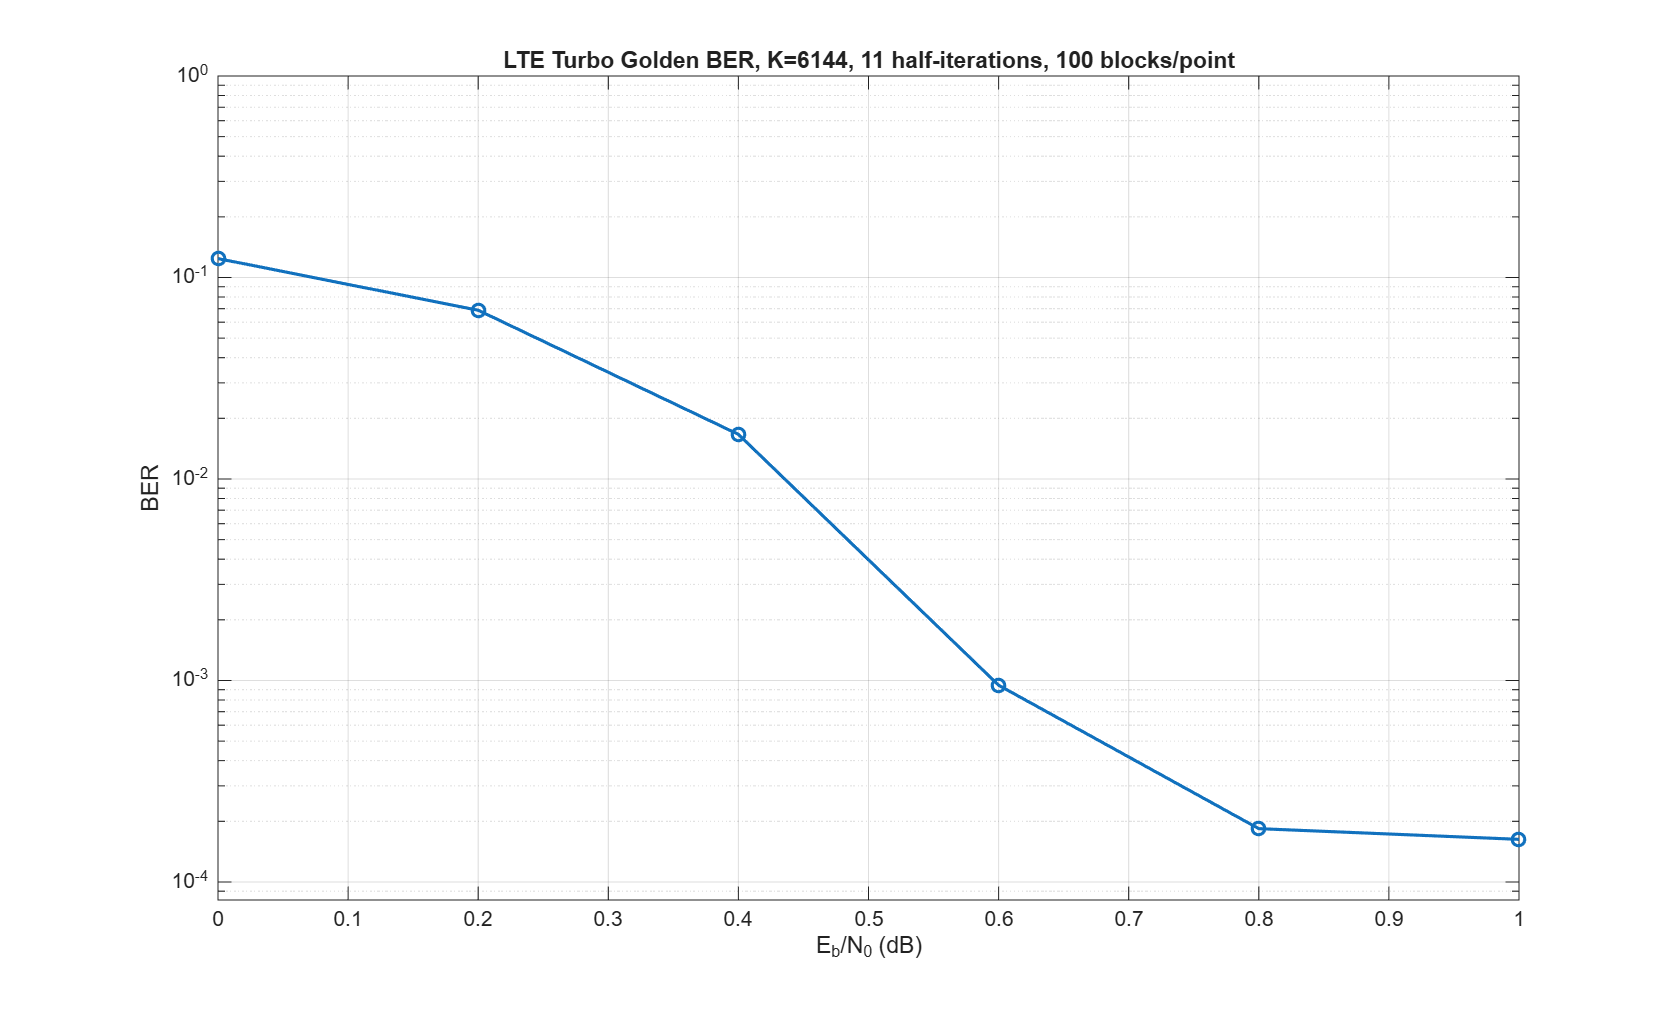
\includegraphics[width=\linewidth]{ber_plot.png}}
\caption{BER vs. Eb/No evaluation characterizing the fixed-point decoding convergence trajectory across the defined waterfall envelope.}
\label{fig:ber_plot}
\end{figure}

As documented in Table~\ref{tab:ber_data} and visualized within Fig.~\ref{fig:ber_plot}, the architectural scaling and fractional offset implementations maintain excellent performance symmetry. Between 0.4 dB and 0.6 dB Eb/No constraints, the decoder aggressively initiates its primary waterfall phase—descending symmetrically from a $1.66 \times 10^{-2}$ BER down strictly into $9.47 \times 10^{-4}$. Marginal returns stabilize towards an estimated error plateau registering at roughly $1.62 \times 10^{-4}$ at 1.0 dB. This successfully validates the algorithmic superiority of the adapted topological simplifications.

\subsection{Comparison with Reference Architectures}
Table~\ref{tab:comparison} juxtaposes the baseline implementation results against the original reference architecture.

\begin{table}[htbp]
\caption{Architecture Implementation Comparison}
\begin{center}
\footnotesize
\begin{tabular}{|l|c|c|}
\hline
\textbf{Metric} & \textbf{This Work (FPGA)} & \textbf{Reference \cite{studer2011} (ASIC)} \\
\hline
Target Tech. & Zynq-7010 (28nm) & 0.13 $\mu$m CMOS \\
\hline
Parallel Cores ($N$) & 2 & 8 \\
\hline
Window Protocol & $W=30$ Radix-4 & $W=30$ Radix-4 \\
\hline
Clock & 100 MHz & 302 MHz \\
\hline
Decode Th. & 39.93 Mbps & 390.6 Mbps \\
\hline
End-to-end Th. & 22.17 Mbps & -- \\
\hline
\end{tabular}
\label{tab:comparison}
\end{center}
\end{table}

\subsection{Discussion}
The throughput difference between this FPGA implementation and the reference ASIC is mainly due to the reduced parallelism and the target technology. This work uses $N=2$ SISO cores, whereas the reference architecture uses $N=8$. For $K=3200$, the interleaved decode phase reaches 39.93 Mbps at 100 MHz, while the end-to-end throughput including eight input-load phases is 22.17 Mbps.

The routed design meets the 100 MHz constraint with 0.230 ns setup WNS and no hold violation. The limiting decoder path remains the DBR ACS-to-ACS chain, where routing delay dominates logic delay.

\section{Conclusion}
This paper presented a dual-SISO radix-4 M-BCJR turbo decoder for $K=3200$ on the Zynq-7010 FPGA. The design meets the 100 MHz clock target and achieves 39.93 Mbps interleaved decode throughput, or 22.17 Mbps end-to-end throughput when input loading is included. The measured latency breakdown confirms the expected 75-cycle window schedule and the additional interleaver routing cost. Further speed improvement should focus on the radix-4 ACS datapath and high-fanout interleaver control logic.

\begin{thebibliography}{00}
\bibitem{studer2011}
C. Studer, C. Benkeser, S. Belfanti, and Q. Huang, ``Design and Implementation of a Parallel Turbo-Decoder ASIC for 3GPP-LTE,'' \textit{IEEE Journal of Solid-State Circuits}, vol. 46, no. 1, pp. 8-21, Jan. 2011.
\end{thebibliography}

\end{document}
